\section{Proposing Private Data Collections For Data Privacy}
\label{pdc}
\textbf{Key Idea.}
To hide the private data from specific members in a blockchain
network, we propose the following:
\begin{enumerate}[topsep=0pt,noitemsep,leftmargin=15pt]
    \item Share and store private data only on a node owned by the member
        who should see the data. To achieve this, we introduce private data
        \textit{collection} with membership. Any data intended for a
        \textit{collection} is stored only on that collection's members' node.
    \item Share and store the hash of private data on all nodes as evidence
        for tamper detection. In other words, store the hash of private data
        (present in each \textit{collection}) on the replicated ledger,
        visible to all members.
\end{enumerate}
% to share the private data only with the members
% who should see it and store the hash of private data on the replicated
% ledger as evidence for tamper detection. To achieve this, we propose
% private data collection with membership---any data stored on a collection is
% visible and reside only on the collection members' node. The hash of
% the private data and any public data get stored on the replicated ledger,
% which is visible to all nodes.
\par
Figure~\ref{fig:fsc-pvt-data-food-traceability} showcases the use of private data collection
to achieve data privacy in the food traceability use-case.
There are five private data collections, where four of them have two members, and the
rest with just one member.
%There are four private data collections, each with two members and one private data
% collection with just one member.
The replicated ledger contains public data such the order IDs, product \& lot IDs, participants
involved in each transaction, and the hash of each private data stored in each collection. For each
order ID, the respective private data such as the order details, invoices, and payment are stored
in a collection depending on who issued the order to whom. Thus, the food traceability solution
achieves data privacy.
\par
Figure~\ref{fig:fsc-pvt-data-health-care} showcases the use of private
data collection to achieve data privacy in the health-care use-case.
There are five private data collections, each with only one member.
A hospital stores its patient's medical record on a collection where the
respective hospital's node is a member.
On an as-needed basis, such as during an insurance claim, a patient can copy
their medical record located at one hospital's collection to another where the
insurance provider is a member. As the medical record evidence (i.e., the record's hash)
is present in the replicated ledger, the receiving party can ensure its authenticity.
Similarly, a patient can copy or move their medical record from one hospital's
collection to another.
% Here, each
% hospital, regulator, and insurance provider owns a private data collection.
% A patient's medical record at one hospital's collection can be copied to another
% collection in which the regulator or insurance provider is a member on an as-needed
% basis. As the medical record evidence, i.e., hash of the record, is present in the
% replicated ledger, the receiving party can ensure the record's authenticity.
% Similarly, a patient's medical record can be copied or moved from one hospital's
% collection to another when the patient shifts.
\par
\textbf{Design Requirements.}
The following requirements should be satisfied with our design to allow a wide variety of use-cases,
including the three use-cases described in \S\ref{motivation}.
\begin{enumerate}[topsep=0pt,noitemsep,leftmargin=15pt]
        \item[\textbf{R1}] As part of the transaction, a client could include a list of collection
            and private data to be stored, accessed, or modified in each collection. A submitted
            transaction should be executed only by a smart-contract hosted on nodes running in a
            blockchain network to ensure the standard data format needed to share data across different
            members and follow the agreed business processes. In other words, only a smart-contract
            can store, access, or modify a private data stored in a collection.
            % As a part of transaction, the client
            % should be able to include the name of collections and private data to be stored, accessed
            % or modified in each of that collection. The transaction submitted to a blockchain network should
            % be executed only by a smart-contract to ensure the standard data format needed for sharing data
            % across different members and following the agreed business processes. In other words, only
            % a smart-contract can store, access, or modify a data stored in a collection.
		% \item[\textbf{R1}] The private data stored on a collection must be accessed or modified
            % through a smart-contract only. The smart-contract ensures the standard data format
            % needed for sharing data across different members and following the agreed business processes.
            % The private data stored on a collection must be accessed or modified through
            % a smart-contract only. The smart-contract helps to ensure common data
            % format needed for sharing data across different members and to follow the agreed business processes.
        \item[\textbf{R2}] A transaction should be executed only on members' node with whom the private data
            is shared. In other words, a smart-contract executing a transaction should have access to all collections
            specified in the transaction and the public data stored on the replicated ledger. Hence,
            a transaction should be allowed to execute only on a subset of nodes in a network because
            a node has access to a collection only if it is a member of that collection.
            % A smart-contract, hosted on nodes running in
            % a blockchain network, that executing the transaction should be able to access all collections
        % specified in the transaction input and the public data stored on the replicated ledger.
        % As a result, the transaction may not be submitted/executed on all members' node because
        % a node can access a collection only if it is a member of that collection.
            % A transaction input needs to include the name of private data collection and
            % private data to be stored or modified. The smart-contract hosted on a blockchain network
            % that processing the transaction should be able to access all private data collections specified
            % in the transaction input as well as the public data stored on the replicated ledger.
            % As a result, the transaction may not be submitted/executed on all nodes in the network.
		\item[\textbf{R3}] When a transaction, executed by smart-contract, modifies both the public and private data,
				the atomicity and serializable isolation should be guaranteed.
		\item[\textbf{R4}] The private data's hash stored on the replicated ledger should always be in sync with the
				actual private data stored in the collection.
		\item[\textbf{R5}] The members of a collection should be mutable, i.e., a new member can be added, or an
            old member can be removed. A newly added member’s node should receive and store all private data in
            that collection, including the existing data. A removed member’s node should have access only to data
            that was persisted when it was a member.
            % The members of a collection should be mutable, i.e., a new member can be added, or an old member can be
            % removed. A newly added member's node should receive and store all private data in that collection
            % including the existing data. A removed member's node should have access only to data that
            % was persisted when it was a member.
		\item[\textbf{R6}] The data stored in a collection can have a time-to-live property.
\end{enumerate}
\begin{figure}
    \begin{center}
	    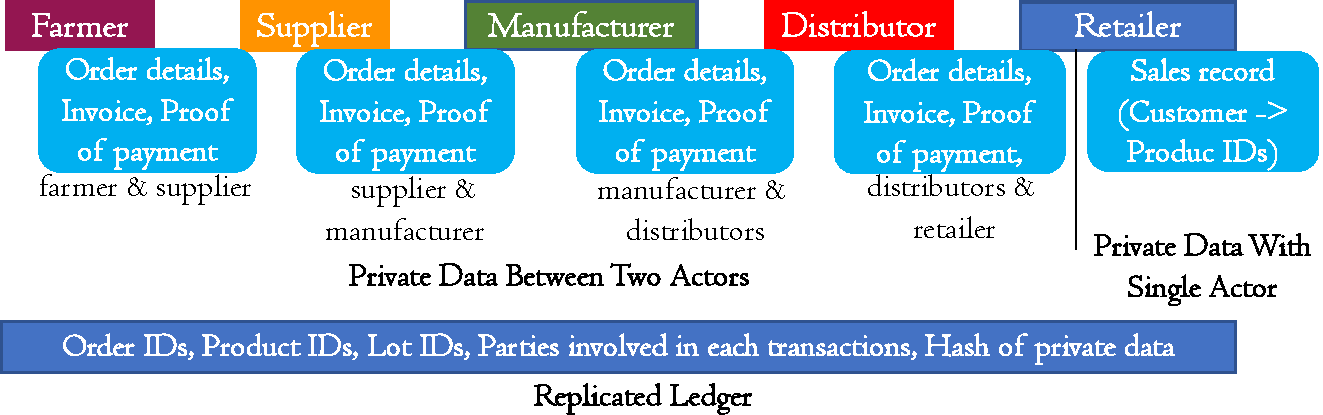
\includegraphics[scale=0.42]{fig/fsc-private-data.pdf}
  		\vspace{-.4cm}
		\caption{\small{The private/sensitive data is visible only to the appropriate parties and the proof of data existance is stored
						in a replicated ledger along with necessary information needed to enable traceability}.}
		\label{fig:fsc-pvt-data-food-traceability}
 \end{center}
  \vspace{-.5cm}
\end{figure}

\begin{figure}
    \begin{center}
			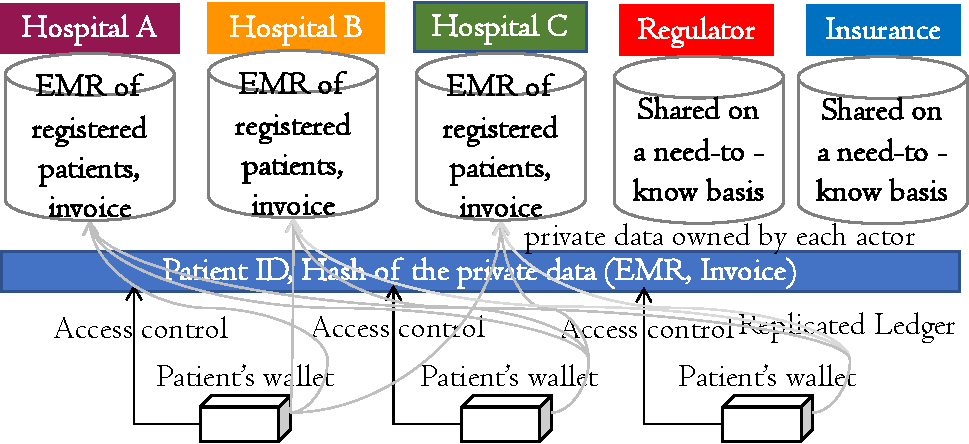
\includegraphics[scale=0.42]{fig/health-care-private-data.pdf}
  		\vspace{-.4cm}
		\caption{\small{The private/sensitive data is maintained at the node of each individual hospital's node and the proof of data
						existance is stored in a replicated ledger along with necessary information needed to share data on a need-to-know basis}.}
		\label{fig:fsc-pvt-data-health-care}
 \end{center}
  \vspace{-.5cm}
\end{figure}
\begin{figure*}
    \begin{center}
	    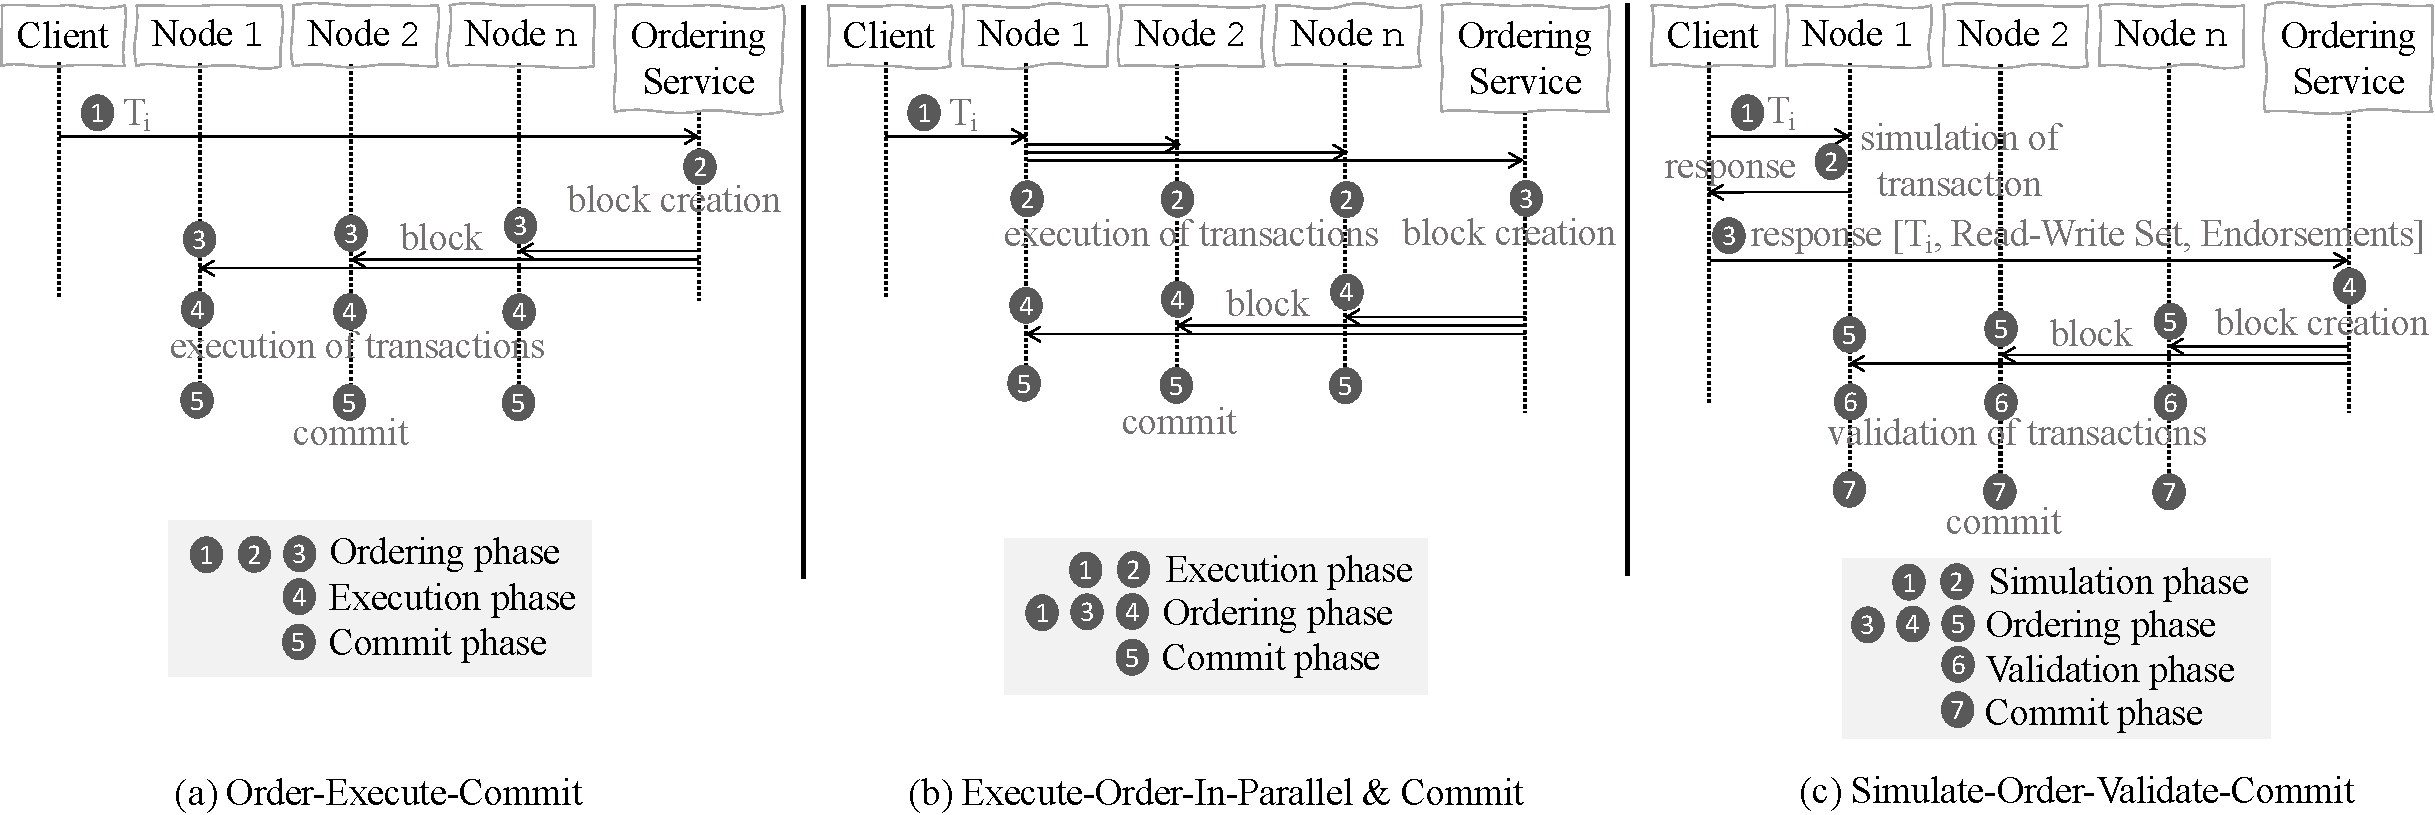
\includegraphics[scale=0.42]{fig/replication-protocol.pdf}
  		\vspace{-.4cm}
        \caption{\small{Blockchain replication protocols}.}
		\label{fig:replication-protocol}
 \end{center}
  \vspace{-.5cm}
\end{figure*}
\section{Implication of Blockchain Replication Protocols on Private Data Collections}
This section considers three existing blockchain replication protocols depicted in Figure~\ref{fig:replication-protocol}
and discusses whether the proposed private data collection can be implemented while satisfying the design requirements specified in 
% §3. 
% In this section, we consider three existing blockchain replication protocols depicited in 
% and discuss whether the proposed private data collection can be implemented while satisfying the design requirements
% specified in 
\S\ref{pdc}. %Note that it is possible to implement requirements R4 and R5 in all three
%existing replication protocols, and hence it is not discussed in this section
Note that in these replication protocols, the identifier or name of the smart-contract
that executes a transaction is specified in the transaction input itself along with the other inputs
required for the execution of contract functions.
\subsection{Order-Execute-Commit} 
\label{order-execute-commit}
Figure~\ref{fig:replication-protocol}(a) presents the three phases, (1) ordering, (2) execution, and (3) commit,
of this replication protocol. In the
ordering phase, first, the user-submitted transactions are ordered, and a block is generated through
mining/consensus. Second, the created block is broadcasted to all nodes in the blockchain network. In the
execution phase, on receiving a block, each node executes transactions present in the block serially by invoking the appropriate
smart-contract. Finally, in the commit phase, the executed transactions are committed.
Ethereum~\cite{}, Quorum~\cite{}, and Hyperledger Besu~\cite{} implement order-execute-commit replication protocol.
In this protocol, the transactions are passed to all nodes via a block. All nodes execute the transactions. Hence, it is not
trivial to support requirement R2 listed in \S\ref{pdc}.
% In this replication protocol, first, the user-submitted transactions are ordered, and a block is generated through
% mining/consensus. Second, the created block is broadcasted to all nodes in the blockchain network. Third, on receiving
% a block, each node executes the transaction serially by invoking the appropriate smart-contract and commit the same.
% Ethereum~\cite{}, Quorum~\cite{}, and Hyperledger Besu~\cite{} implements order-execute-commit replication protocol.
% In this protocol, the transaction input are passed to all nodes via a block. All nodes execute the smart-contract
% using the input. Hence, it is not possible to support requirement R1 listed in \S\ref{pdc} with this protocol.
% Given that transaction input go to all nodes, we need to pass the private data to members' node via
% a separate mechanism and only pass the hashed state in the transaction input. However, with this solution, it
% is not possible to support requirements R1, R2, and R3 listed in \S\ref{pdc}. The requirement R1 cannot be satisfied
% because the smart-contract is executed on all nodes, i.e., even on the nodes which do not have access to the required
% private data collection.
% The requirement R2 cannot be satisfied as we need to store the private data separately before or after storing the hash
% on the replicated ledger using the smart-contract.
% The requirement R3 cannot be satisfied because the user cannot pass the pointer to the private
% data, such as order ID, in the transaction input that needs to be modified as it would reveal some information
% about the private data.
% Given these drawbacks, we decide not to pick the blockchain platforms
% which support only the order-execute-commit replication protocol.
\subsection{Execute-Order-In-Parallel \& Commit}
Figure~\ref{fig:replication-protocol}(b) presents the three phases, (1) execution, (2) ordering, and (3) commit,
of this replication protocol.
In the execution phase, submitted transactions are executed in parallel on nodes without prior knowledge of order,
while the ordering phase happens simultaneously through a consensus service or mining. Once the block is created and
delivered to nodes, the executed transactions would get committed/aborted depending on the commit phase's serializability
check. The BlockchainRDBMS~\cite{} implements this replication protocol. Similar to the order-execute-commit protocol,
it is not trivial to satisfy requirements R2.
% In the execution phase, submitted transactions are executed in parallel on nodes without prior knowledge of ordering
% while ordering phase happens simultaneously through a consensus service or mining. Once the block is created and
% delivered to nodes, the executed transactions would get committed/aborted depending on the serializability check
% in the commit phase.
% If a node never received a transaction that is present in the block, it would execute the transaction and commit.
% The BlockchainRDBMS~\cite{} implements this replication protocol. Similar to the
% order-execute-commit protocol, it is not trivial to satisfy requirements R2.
\subsection{Execute-Order-Validate-Commit.}
Figure~\ref{fig:replication-protocol}(c) presents the four phases, (1) execution, (2) ordering, (3) validation, and
(4) commit, of this replication protocol.
In the execution phase, the transaction is executed on a sub-set
of nodes depending on the endorsement policy defined for a smart-contract. As a result of transaction execution,
the read-write set is collected. In the ordering phase, the read-write set and
endorsements are sent to the consensus service for transaction ordering and block creation. Once the block is created,
it is delivered to all nodes in the blockchain network. In the validation phase, on receiving the block, each node verifies whether
the transaction has collected enough endorsements as per the policy defined for the invoked smart-contract and executes
Optimistic Concurrency Control~\cite{} using the read-write set to perform serializability check. Finally, in the commit phase,
only valid serializable transactions are committed. Hyperledger Fabric~\cite{} implements execute-order-validate-commit
replication protocol.
% \par
We can implement private data collection with this replication protocol while satisfying all six requirements
mentioned in \S\ref{pdc} as shown in \S\ref{}.
% To satisfy requirement R1 and R2, we can pass the private data in the transaction input itself
% and simulate the transaction only on nodes which are the members of the private data collection. To ensure that
% only members stores the private data, during transaction simulation, we can store the private data in a temporary store
% and include only the hash of private data in the read-write set which goes to all nodes via a block for validation
% and commit. During commit, for valid transactions, we can fetch the corresponding private data from the temporary store.
% Thus, the requirements R3 and R4 are satisfied. The other requirements can also be satisfied as shown in \S\ref{}.
% Given that transaction can be simulated on a sub-set of nodes, we can pass the private
% data in the transaction input itself and simulate the transaction as per the collection membership. Thus, the
% smart-contract can access both private and public states which satisfies the requirement R1. As the simulation
% result includes read-write set, we can make the node to compute and store only the hash of private data in the
% read-write set which goes to all node to get stored in the replicated ledger. During transaction simulation,
% we can store the private data in a temporary store and fetch it while processing the read-write set during the
% commit time. Thus, we can satisfy requirements R2 and R3.
